\documentclass[12pt,a4paper]{article}

% Packages
\usepackage[utf8]{inputenc}
\usepackage[T1]{fontenc}
\usepackage{lmodern}
\usepackage[margin=1in,headheight=15pt]{geometry}
\usepackage{graphicx}
\usepackage{tikz}
\usetikzlibrary{shapes.geometric, arrows.meta, positioning, fit, backgrounds, calc}
\usepackage{listings}
\usepackage{xcolor}
\usepackage{hyperref}
\usepackage{booktabs}
\usepackage{float}
\usepackage{caption}
\usepackage{subcaption}
\usepackage{amsmath}
\usepackage{enumitem}
\usepackage{fancyhdr}
\usepackage{titlesec}

% Colors
\definecolor{codegreen}{rgb}{0,0.6,0}
\definecolor{codegray}{rgb}{0.5,0.5,0.5}
\definecolor{codepurple}{rgb}{0.58,0,0.82}
\definecolor{backcolour}{rgb}{0.95,0.95,0.92}
\definecolor{meluxinaBlue}{RGB}{0,102,179}
\definecolor{serverGreen}{RGB}{76,175,80}
\definecolor{clientOrange}{RGB}{255,152,0}
\definecolor{monitorPurple}{RGB}{156,39,176}
\definecolor{discoveryTeal}{RGB}{0,150,136}

% Code listing style
\lstdefinestyle{mystyle}{
    backgroundcolor=\color{backcolour},   
    commentstyle=\color{codegreen},
    keywordstyle=\color{magenta},
    numberstyle=\tiny\color{codegray},
    stringstyle=\color{codepurple},
    basicstyle=\ttfamily\footnotesize,
    breakatwhitespace=false,         
    breaklines=true,                 
    captionpos=b,                    
    keepspaces=true,                 
    numbers=left,                    
    numbersep=5pt,                  
    showspaces=false,                
    showstringspaces=false,
    showtabs=false,                  
    tabsize=2
}
\lstset{style=mystyle}

% YAML language definition
\lstdefinelanguage{yaml}{
    keywords={true,false,null,y,n},
    sensitive=false,
    comment=[l]{\#},
    morestring=[b]',
    morestring=[b]"
}

% JSON language definition
\lstdefinelanguage{json}{
    string=[s]{"}{"}, 
    comment=[l]{//},
    morecomment=[s]{/*}{*/},
    literate=
     *{0}{{{\color{blue}0}}}{1}
      {1}{{{\color{blue}1}}}{1}
      {2}{{{\color{blue}2}}}{1}
      {3}{{{\color{blue}3}}}{1}
      {4}{{{\color{blue}4}}}{1}
      {5}{{{\color{blue}5}}}{1}
      {6}{{{\color{blue}6}}}{1}
      {7}{{{\color{blue}7}}}{1}
      {8}{{{\color{blue}8}}}{1}
      {9}{{{\color{blue}9}}}{1}
}

% Header/Footer
\pagestyle{fancy}
\fancyhf{}
\lhead{EUMaster4HPC Student Challenge 2025}
\rfoot{Page \thepage}

% Hyperref setup
\hypersetup{
    colorlinks=true,
    linkcolor=meluxinaBlue,
    filecolor=magenta,      
    urlcolor=cyan,
    pdftitle={Benchmarking AI Factories on MeluXina Supercomputer},
}

\title{
    \vspace{-1cm}
    \textbf{Benchmarking AI Factories on MeluXina Supercomputer}\\
    \large A Unified Platform for Deploying, Monitoring, and Benchmarking\\
    AI Factories\\
    \vspace{0.5cm}
    \normalsize EUMaster4HPC Student Challenge 2025
}

\author{
    Tommaso Crippa\\
    Edoardo Leali\\
    Emanuele Caruso\\
    \vspace{0.5cm}\\
    Supervisor: Dr Farouk Mansouri
}

\date{12 January 2026}


\begin{document}

\maketitle

\begin{abstract}
This report presents our implementation for the EUMaster4HPC Student Challenge 2025, where we were tasked to build a unified framework designed to streamline the deployment, monitoring, and benchmarking of AI inference services on High-Performance Computing clusters. The framework addresses the challenges of managing containerized AI workloads in SLURM-based environments. Our application provides three integrated modules (Server, Monitor, and Client) that work together through an automatic service discovery mechanism. The framework enables researchers and engineers to deploy inference servers, monitor performance metrics via Prometheus, and execute standardized benchmarks with minimal manual configuration. This report details the system architecture, design decisions, implementation specifics, and provides guidance on deploying the framework on the MeluXina supercomputer.
\end{abstract}

\tableofcontents
\newpage

%==============================================================================
\section{Introduction}
%==============================================================================

\subsection{The Rise of AI Factories}

The artificial intelligence landscape is undergoing a fundamental transformation with the emergence of AI Factories, large-scale inference platforms designed to serve AI models at production scale. Unlike traditional research-focused deployments, AI Factories represent the industrialization of AI, where models must deliver consistent, low-latency responses to thousands of concurrent users while maintaining cost efficiency and reliability.

This shift from experimentation to production has been driven by multiple interconnected factors. The explosion of \textbf{foundation models}, including large language models, vision models, and multimodal systems, has created unprecedented demand for specialized inference infrastructure capable of handling production workloads. Organizations across industries are moving beyond proof-of-concept deployments and adopting AI in more and more scenarios, requiring robust infrastructure with enterprise-grade reliability. The \textbf{scale requirements} have grown dramatically, with single inference endpoints now expected to serve millions of requests daily. At the same time, there is mounting pressure to optimize \textbf{GPU utilization} and reduce inference costs, as infrastructure budgets become increasingly constrained. These factors combined have transformed AI from a research curiosity into a production engineering problem.

HPC-based AI Factories need a unified framework that simplifies SLURM integration while preserving access to important HPC features. The framework must provide automatic service discovery in dynamic environments where node assignments change with each deployment. It should collect HPC-specific monitoring metrics beyond standard cloud benchmarks. The system must make benchmarks reproducible through declarative configuration files that can be version-controlled and shared among researchers. Finally, it needs to bridge the gap between cloud AI tools and HPC infrastructure, bringing modern AI development practices to supercomputers while respecting the unique constraints and opportunities that HPC environments offer.

\subsection{Project Goals}

The framework provides a \textbf{unified command-line interface} that handles server deployment, monitoring, and benchmarking through a single consistent tool. It \textbf{eliminates manual endpoint management} through automatic service discovery, removing the need to manually track and configure service addresses. The system enables \textbf{recipe-based configuration} that makes deployments reproducible and shareable across teams. It fully \textbf{supports GPU-accelerated inference servers} on HPC clusters, taking advantage of supercomputer hardware for AI workloads. \textbf{Prometheus monitoring is integrated} with automatic target resolution, so that metric collection is set up without manual configuration. Finally, the framework \textbf{facilitates performance benchmarking} with configurable workload patterns, allowing researchers to test their systems under diverse conditions.

\subsection{Target Platform: MeluXina}

MeluXina is Luxembourg's national supercomputer, featuring AMD EPYC processors and NVIDIA A100 GPUs. The framework is specifically designed to work with the \textbf{SLURM workload manager} for job scheduling, which is the standard scheduler on HPC systems. It uses \textbf{Apptainer} (formerly Singularity) for secure containerization of inference workloads. The system integrates with the \textbf{module system} for managing software environments across different compute nodes.

%==============================================================================
\section{System Architecture}
%==============================================================================

The project follows a modular architecture with three core modules and a central service discovery mechanism. Figure~\ref{fig:architecture} illustrates the high-level system design.

\begin{figure}[H]
\centering
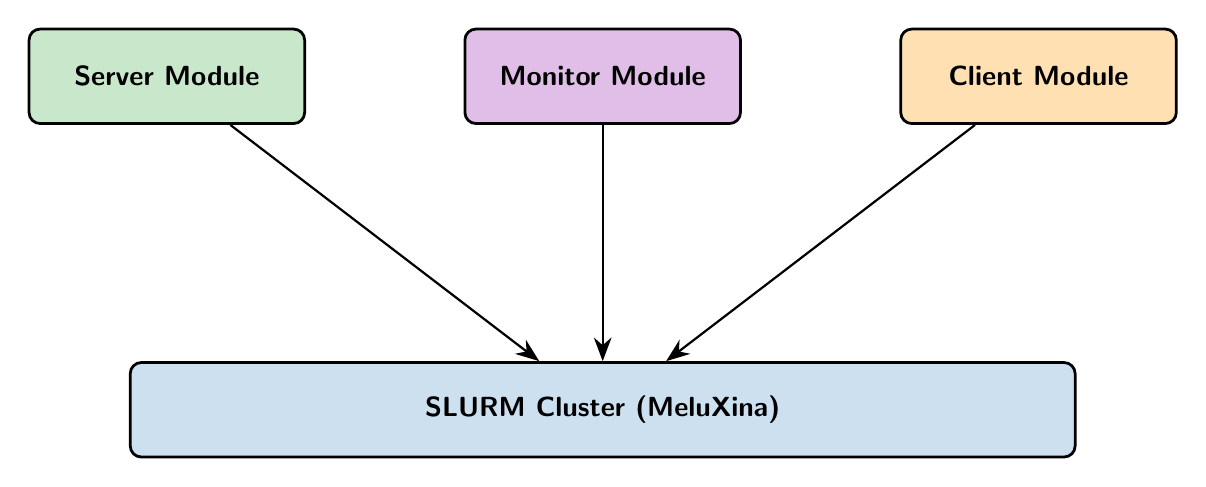
\begin{tikzpicture}[
    node distance=1.5cm and 2cm,
    module/.style={rectangle, rounded corners, draw=black, line width=1pt, minimum width=3.5cm, minimum height=1.2cm, font=\sffamily\bfseries},
    component/.style={rectangle, draw=gray, fill=white, minimum width=2.8cm, minimum height=0.8cm, font=\sffamily\small},
    arrow/.style={-{Stealth[length=3mm]}, thick},
    dasharrow/.style={-{Stealth[length=3mm]}, thick, dashed}
]

% Core Modules
\node[module, fill=serverGreen!30] (server) {Server Module};
\node[module, fill=monitorPurple!30, right=of server] (monitor) {Monitor Module};
\node[module, fill=clientOrange!30, right=of monitor] (client) {Client Module};

% SLURM Layer
\node[module, fill=meluxinaBlue!20, below=3cm of monitor, minimum width=12cm] (slurm) {SLURM Cluster (MeluXina)};
\draw[arrow] (server) -- (slurm);
\draw[arrow] (monitor) -- (slurm);
\draw[arrow] (client) -- (slurm);
\end{tikzpicture}
\caption{High-Level Architecture}
\label{fig:architecture}
\end{figure}

\subsection{Architectural Principles}

The framework is built on several key architectural principles that guide its design and implementation. \textbf{Separation of Concerns} ensures that each module handles a specific domain (deployment, monitoring, benchmarking) with clear interfaces, making the codebase maintainable and easier to extend. \textbf{Recipe-Based Configuration} means that all operations are driven by YAML recipes rather than imperative code, enabling reproducibility and version control of deployments. The \textbf{Manager-Orchestrator Pattern} is used throughout the framework, where each module has a Manager class that handles business logic and an Orchestrator class that interacts directly with SLURM, providing clean separation between domain logic and infrastructure details. \textbf{Automatic Discovery} allows services to register their endpoints automatically as they deploy, eliminating manual configuration propagation and reducing operational overhead.

\subsection{Directory Structure}

The framework organizes code and configuration as follows:

\begin{lstlisting}[language=bash, caption={Project Directory Structure}]
root/
|-- src/
|   |-- server/          # Server deployment module
|   |-- monitor/         # Prometheus monitoring module
|   |-- client/          # Benchmark client module
|   |-- discover.py      # Service discovery mechanism
|   |-- list_services.py # CLI for listing services
|   +-- clear_services.py
|-- recipes/
|   |-- servers/         # Server deployment recipes
|   |-- monitors/        # Monitor configuration recipes
|   +-- clients/         # Benchmark workload recipes
|-- config/
|   +-- slurm.yml        # SLURM configuration defaults
|-- logs/                # Runtime logs and state
+-- results/             # Benchmark output files
\end{lstlisting}



%==============================================================================
\section{Server Module}
%==============================================================================

The Server Module is responsible for deploying AI inference services as SLURM jobs using containerized applications. It provides automated deployment, lifecycle management, and service discovery integration.

\subsection{Module Architecture}

The server module follows a layered architecture with five core classes working together to manage the complete deployment lifecycle. Figure~\ref{fig:server-module} illustrates the relationships between these components.

\begin{figure}[H]
\centering
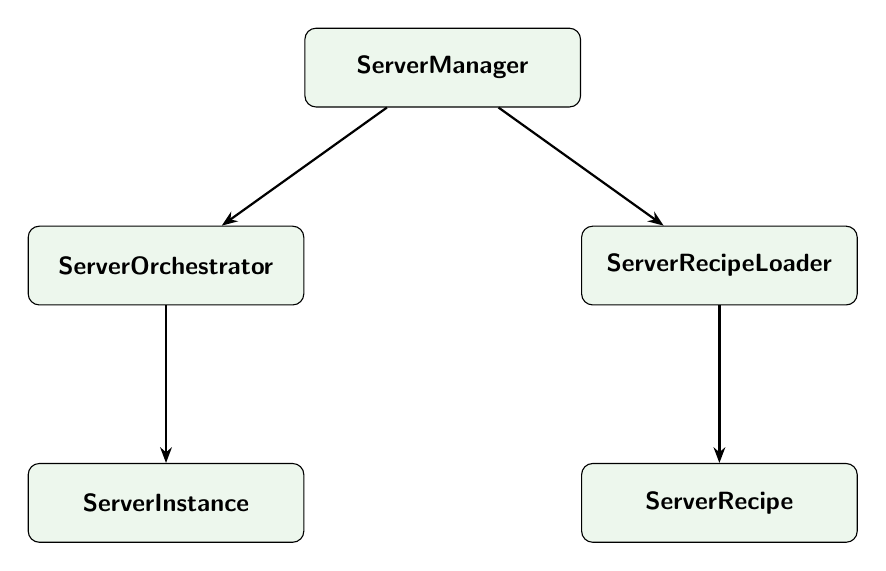
\begin{tikzpicture}[
    node distance=1cm and 1.5cm,
    class/.style={rectangle, draw, rounded corners, fill=serverGreen!10, minimum width=3.5cm, minimum height=1cm, font=\sffamily\small},
    method/.style={font=\ttfamily\tiny, align=left},
    arrow/.style={-{Stealth[length=2mm]}, thick}
]

\node[class] (manager) {\textbf{ServerManager}};
\node[class, below left=1.5cm and 0cm of manager] (orchestrator) {\textbf{ServerOrchestrator}};
\node[class, below right=1.5cm and 0cm of manager] (loader) {\textbf{ServerRecipeLoader}};
\node[class, below=2cm of orchestrator] (instance) {\textbf{ServerInstance}};
\node[class, below=2cm of loader] (recipe) {\textbf{ServerRecipe}};

\draw[arrow] (manager) -- (orchestrator);
\draw[arrow] (manager) -- (loader);
\draw[arrow] (loader) -- (recipe);
\draw[arrow] (orchestrator) -- (instance);

\end{tikzpicture}
\caption{Server Module Class Structure}
\label{fig:server-module}
\end{figure}

\subsection{Class Descriptions}

\subsubsection{ServerManager}

The \texttt{ServerManager} class serves as the primary interface for all server operations, coordinating recipe loading, job submission, and instance lifecycle management. This class implements the high-level business logic while delegating infrastructure concerns to the orchestrator.

The manager maintains a collection of active server instances indexed by unique names. When deploying a server, it loads the recipe specification, creates a \texttt{ServerInstance} object, submits the job through the orchestrator, and waits for SLURM to assign a compute node. Once the node assignment is complete, the manager writes discovery information to the shared filesystem, enabling clients and monitors to automatically locate the service. The synchronous waiting behavior ensures that discovery data is accurate before the deployment operation returns to the user.

Key methods include \texttt{run(recipe\_name, count)} which deploys one or more instances of a server recipe, \texttt{stop(name)} which cancels a running deployment and clears discovery information, \texttt{stop\_all()} which terminates all managed instances, and \texttt{collect\_status()} which queries SLURM for current job states and updates discovery data for running services.

\subsubsection{ServerOrchestrator}

The \texttt{ServerOrchestrator} class handles all direct interaction with the SLURM workload manager, encapsulating platform-specific details and providing a clean abstraction for the manager. This separation enables the framework to support alternative schedulers in the future without modifying business logic.

The orchestrator dynamically generates SBATCH scripts based on recipe specifications, incorporating resource requirements, environment variables, and startup commands. It reads SLURM configuration from environment variables and YAML files, supporting flexible deployment across different HPC systems. The generated scripts include comprehensive logging that records job metadata, node assignments, and execution status.

Core responsibilities include \texttt{submit(instance, recipe)} which builds and submits SBATCH scripts returning job IDs, \texttt{stop(job\_id)} which cancels running jobs using \texttt{scancel}, and \texttt{status(job\_id)} which queries job state using \texttt{squeue} and parses output to determine if jobs are pending, running, or completed. The orchestrator maps SLURM status strings to internal \texttt{ServerStatus} enum values, providing a consistent state model across the framework.

\subsubsection{ServerInstance}

The \texttt{ServerInstance} class represents a single deployed server with runtime state tracking. Each instance receives a unique UUID identifier on creation and maintains a reference to its SLURM job ID (orchestrator handle). The instance tracks its lifecycle status through the \texttt{ServerStatus} enumeration, which includes states such as SUBMITTED, STARTING, RUNNING, COMPLETED, FAILED, and CANCELED.

Instances store deployment metadata including the assigned compute node, exposed ports, creation timestamp, and completion timestamp. This information is essential for service discovery and debugging. 


\subsubsection{ServerRecipe}

The \texttt{ServerRecipe} class represents a parsed and validated server deployment specification loaded from YAML files. Each recipe encapsulates all information needed to deploy a service, including the service startup command, port mappings, environment variables, working directory, and resource requirements.

The recipe validates its configuration during initialization, ensuring that required fields are present and that port numbers fall within valid ranges. It provides convenient property accessors for common configuration elements such as \texttt{resources} which returns the orchestration resource dictionary, \texttt{env} which returns environment variables, \texttt{working\_directory} which specifies where the service executes, and \texttt{ports} which lists exposed network ports.

The class method \texttt{from\_yaml(yaml\_path)} implements the factory pattern for loading recipes from disk, reading YAML files, parsing their contents, and constructing validated recipe objects. This approach centralizes parsing logic and ensures consistent validation across all recipe loads.

\subsubsection{ServerRecipeLoader}

The \texttt{ServerRecipeLoader} class manages recipe discovery, loading, and caching from the recipes directory. It maintains an in-memory cache of loaded recipes to avoid repeated file I/O and parsing overhead. The loader scans the configured recipe directory for YAML files with \texttt{.yml} or \texttt{.yaml} extensions.

Key methods include \texttt{load\_recipe(name)} which locates, parses, and caches a recipe by name, \texttt{list\_available\_recipes()} which returns all recipe names found in the directory, and \texttt{get\_recipe\_info(name)} which returns summary information about a recipe without fully loading it. The loader also provides \texttt{create\_recipe\_template(name)} which generates a starter recipe file with example configuration, helping users create new recipes quickly.

\subsection{Server Recipe Specification}

Server recipes define all aspects of a deployment:

\begin{lstlisting}[language=yaml, caption={vLLM Server Recipe Example}]
name: vllm-server
service_name: vllm
description: vLLM inference server for MeluXina

service:
  command: |
    #!/bin/bash
    module load Apptainer/1.3.6-GCCcore-13.3.0
    
    IMAGE=$CONTAINER_DIR/vllm-openai_v0.5.4.sif
    
    apptainer exec --nv $IMAGE \
      python -m vllm.entrypoints.openai.api_server \
        --model facebook/opt-125m \
        --host 0.0.0.0 \
        --port 8000
  
  working_dir: .
  ports:
    - 8000

orchestration:
  resources:
    cpu_cores: 8
    memory_gb: 64
    gpu_count: 1
    partition: gpu
    time_limit: "04:00:00"
\end{lstlisting}

\subsection{Deployment Workflow}

The server deployment follows this sequence:

\begin{enumerate}
    \item User executes: \texttt{python -m src.server run --recipe vllm-server}
    \item \texttt{ServerManager} loads the recipe from \texttt{recipes/servers/}
    \item A new \texttt{ServerInstance} is created with a unique ID
    \item \texttt{ServerOrchestrator} generates and submits the SBATCH script
    \item Manager polls SLURM until the job is running and node is assigned
    \item Discovery information is written to \texttt{\textasciitilde/.aibenchmark/discover/vllm.json}
    \item Instance is registered and status is returned to user
\end{enumerate}



%==============================================================================
\section{Client Module}
%==============================================================================

The Client Module executes benchmarks against deployed AI services, collecting performance metrics and generating comprehensive reports. It supports multiple workload patterns and provides detailed latency and throughput measurements.

\subsection{Module Architecture}

The client module consists of six core classes that work together to execute benchmarks as SLURM jobs. Figure~\ref{fig:client-module} shows the architectural relationships.

\begin{figure}[H]
\centering
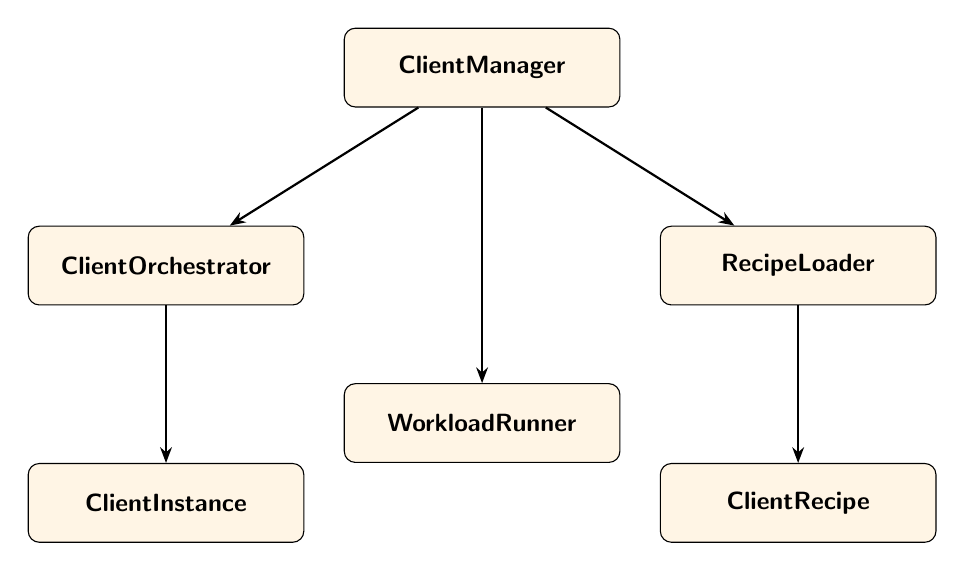
\begin{tikzpicture}[
    node distance=1cm and 1.5cm,
    class/.style={rectangle, draw, rounded corners, fill=clientOrange!10, minimum width=3.5cm, minimum height=1cm, font=\sffamily\small},
    arrow/.style={-{Stealth[length=2mm]}, thick}
]

\node[class] (manager) {\textbf{ClientManager}};
\node[class, below left=1.5cm and 0.5cm of manager] (orchestrator) {\textbf{ClientOrchestrator}};
\node[class, below right=1.5cm and 0.5cm of manager] (loader) {\textbf{RecipeLoader}};
\node[class, below=2cm of orchestrator] (instance) {\textbf{ClientInstance}};
\node[class, below=2cm of loader] (recipe) {\textbf{ClientRecipe}};
\node[class, below=3.5cm of manager] (runner) {\textbf{WorkloadRunner}};

\draw[arrow] (manager) -- (orchestrator);
\draw[arrow] (manager) -- (loader);
\draw[arrow] (loader) -- (recipe);
\draw[arrow] (manager) -- (runner);
\draw[arrow] (orchestrator) -- (instance);

\end{tikzpicture}
\caption{Client Module Class Structure}
\label{fig:client-module}
\end{figure}

\subsection{Class Descriptions}

\subsubsection{ClientManager}

The \texttt{ClientManager} class serves as the primary interface for benchmark operations, coordinating recipe loading, service discovery, and benchmark execution. This manager maintains a collection of active benchmark runs and provides methods for executing single or multiple benchmark iterations.

The manager integrates with the service discovery mechanism to automatically locate target services. When a benchmark recipe specifies a service name, the manager reads discovery information to determine the current endpoint, eliminating manual endpoint configuration. This integration enables seamless benchmarking workflows where users can deploy servers and immediately run benchmarks against them without copying connection details.

Key methods include \texttt{run\_bench(name, runs)} which loads a recipe, discovers the target endpoint, and executes one or more benchmark runs, \texttt{add\_client(name, config)} which manually registers a client configuration, \texttt{remove\_client(name)} which unregisters a client and cancels running benchmarks, \texttt{stop\_all()} which terminates all active benchmark jobs, and \texttt{collect\_metrics()} which gathers performance metrics from all client instances for analysis.

\subsubsection{ClientOrchestrator}

The \texttt{ClientOrchestrator} class handles SLURM integration for benchmark jobs, generating SBATCH scripts and managing job submission. Similar to the server orchestrator, this class encapsulates scheduler-specific logic and provides a clean abstraction for the manager.

The orchestrator builds batch scripts that invoke the workload runner with appropriate parameters derived from the recipe configuration. It handles both closed-loop and open-loop workload patterns, constructing command-line arguments for duration, concurrency, think time, and request payloads. The orchestrator also manages resource allocation, ensuring benchmark jobs receive sufficient CPU and memory to generate their target workload without becoming resource-constrained.

Core responsibilities include \texttt{submit(run, recipe, target\_endpoint)} which generates and submits benchmark jobs, \texttt{stop(job\_id)} which cancels running benchmarks using \texttt{scancel}, \texttt{status(job\_id)} which queries SLURM for job state. The orchestrator also handles payload generation from dataset specifications, supporting both synthetic datasets defined inline and custom datasets loaded from files.

\subsubsection{ClientInstance}

The \texttt{ClientInstance} class represents a single benchmark run with state tracking and metrics collection. Each instance receives a unique identifier and maintains a reference to its SLURM job ID. The instance tracks its lifecycle through the \texttt{RunStatus} enumeration with states including SUBMITTED, RUNNING, COMPLETED, FAILED, and CANCELED.

Instances store benchmark results as they complete, including total requests, success counts, error counts, latency measurements, and throughput calculations. The class provides lifecycle methods including \texttt{start()} which transitions to RUNNING state, \texttt{stop()} which cancels the benchmark, and \texttt{update\_status(new\_status)} which transitions the instance through states.

Metrics methods support result reporting and analysis. The \texttt{get\_metrics()} method returns a comprehensive dictionary including run identifier, recipe name, status, duration, endpoint, and all collected performance metrics. The \texttt{to\_dict()} method provides JSON serialization for persistence and logging.

\subsubsection{ClientRecipe}

The \texttt{ClientRecipe} class represents a parsed benchmark specification loaded from YAML files. Each recipe defines the target service, workload pattern, dataset configuration, resource requirements, and output settings. The recipe validates its configuration during initialization, checking for required fields and ensuring that parameters fall within valid ranges.

The recipe supports both service discovery and explicit endpoint specification. When a \texttt{service\_name} field is present, the framework attempts service discovery before falling back to explicit endpoints. This flexibility enables both automatic and manual configuration workflows.

Key properties include \texttt{target} which specifies protocol and endpoint configuration, \texttt{workload} which defines pattern, duration, concurrency, and think time, \texttt{dataset} which configures request payloads including prompt length, token limits, and model parameters, \texttt{orchestration} which specifies SLURM resources, and \texttt{output} which controls metrics collection and result destination.

The class method \texttt{from\_yaml(yaml\_path)} implements recipe loading from disk, parsing YAML content and constructing validated recipe objects. The \texttt{validate()} method ensures configuration correctness before benchmarks execute.

\subsubsection{WorkloadRunner}

The \texttt{WorkloadRunner} class implements the actual benchmark execution logic, generating HTTP requests and measuring performance. This class runs directly on SLURM compute nodes as part of benchmark jobs, making requests to target services and collecting latency data.

The runner supports two workload patterns. \textbf{Closed-loop mode} simulates realistic user behavior by maintaining a fixed number of concurrent users with think time between requests. Each user makes requests sequentially, waiting for responses before issuing the next request. This pattern tests how systems behave under user-driven load. \textbf{Open-loop mode} generates requests at a constant rate regardless of response times, useful for stress testing and finding maximum throughput limits. This pattern can drive systems beyond their capacity, revealing failure modes and queueing behavior.

For each request, the runner measures end-to-end latency including network time, records HTTP status codes, and tracks success or failure. After the benchmark completes, the runner computes aggregate statistics including total requests, success count, error count, average latency, minimum latency, maximum latency, and throughput in requests per second. These metrics are written to JSON files for analysis.

Core methods include \texttt{run()} which executes the benchmark and returns metrics, \texttt{\_run\_closed\_loop()} which implements concurrent user simulation, \texttt{\_run\_open\_loop()} which implements fixed-rate request generation, \texttt{\_make\_request()} which executes individual HTTP requests with error handling, and \texttt{\_compute\_metrics(total\_duration)} which calculates aggregate performance statistics from collected measurements.

\subsubsection{RecipeLoader}

The \texttt{RecipeLoader} class manages client recipe discovery, loading, and caching. It scans the recipes directory for YAML files and maintains an in-memory cache to avoid repeated parsing. The loader provides \texttt{load\_recipe(name)} for loading specific recipes, \texttt{list\_available\_recipes()} for discovering all available benchmarks, and caching mechanisms for performance optimization.

\subsection{Workload Patterns}

The framework supports two workload patterns:

\subsubsection{Closed-Loop Pattern}

Simulates real users with think time between requests:

\begin{lstlisting}[language=yaml]
workload:
  pattern: closed-loop
  concurrent_users: 10
  think_time_ms: 500      # 500ms delay between requests
  requests_per_user: 100
  duration_seconds: 300
\end{lstlisting}

\subsubsection{Open-Loop Pattern}

Generates requests at a fixed rate regardless of response times:

\begin{lstlisting}[language=yaml]
workload:
  pattern: open-loop
  requests_per_second: 50
  duration_seconds: 300
\end{lstlisting}


\subsection{Collected Metrics}

\begin{table}[H]
\centering
\caption{Benchmark Output Metrics}
\begin{tabular}{ll}
\toprule
\textbf{Metric} & \textbf{Description} \\
\midrule
\texttt{total\_requests} & Total requests made \\
\texttt{successes} & Successful requests (2xx status) \\
\texttt{errors} & Failed requests \\
\texttt{avg\_latency\_ms} & Average latency \\
\texttt{min\_latency\_ms} & Minimum latency \\
\texttt{max\_latency\_ms} & Maximum latency \\
\texttt{throughput\_req\_per\_sec} & Requests per second \\
\bottomrule
\end{tabular}
\end{table}

%==============================================================================
\section{Monitor Module}
%==============================================================================

The Monitor Module deploys Prometheus monitoring stacks to collect metrics from running AI services. It provides automatic target discovery, metrics export capabilities, and service-specific metric selection.

\subsection{Module Architecture}

The monitor module implements a sophisticated monitoring infrastructure with eight core classes managing the complete Prometheus lifecycle. Figure~\ref{fig:monitor-module} illustrates component relationships.

\begin{figure}[H]
\centering
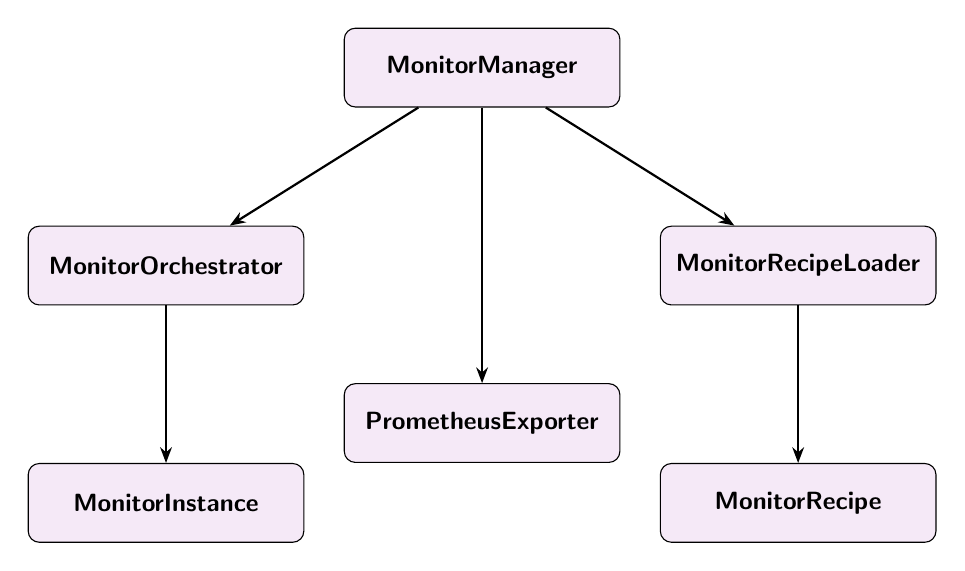
\begin{tikzpicture}[
    node distance=1cm and 1.5cm,
    class/.style={rectangle, draw, rounded corners, fill=monitorPurple!10, minimum width=3.5cm, minimum height=1cm, font=\sffamily\small},
    method/.style={font=\ttfamily\tiny, align=left},
    arrow/.style={-{Stealth[length=2mm]}, thick}
]

\node[class] (manager) {\textbf{MonitorManager}};

\node[class, below left=1.5cm and 0.5cm of manager] (orchestrator) {\textbf{MonitorOrchestrator}};

\node[class, below=3.5cm of manager] (exporter) {\textbf{PrometheusExporter}};

\node[class, below right=1.5cm and 0.5cm of manager] (loader) {\textbf{MonitorRecipeLoader}};

\node[class, below=2cm of loader] (recipe) {\textbf{MonitorRecipe}};

\node[class, below=2cm of orchestrator] (instance) {\textbf{MonitorInstance}};


\draw[arrow] (manager) -- (orchestrator);
\draw[arrow] (manager) -- (exporter);
\draw[arrow] (manager) -- (loader);
\draw[arrow] (orchestrator) -- (instance);
\draw[arrow] (loader) -- (recipe);

\end{tikzpicture}
\caption{Monitor Module Class Structure}
\label{fig:monitor-module}
\end{figure}

\subsection{Class Descriptions}

\subsubsection{MonitorManager}

The \texttt{MonitorManager} class orchestrates the complete monitoring lifecycle, managing Prometheus deployments, target resolution, and metrics export operations. This manager maintains persistent state across sessions by saving instance information to JSON files in the logs directory, enabling recovery after framework restarts.

The manager integrates deeply with the service discovery mechanism. When starting a monitor, it reads discovery information for target services and automatically resolves their endpoints. This eliminates manual configuration of Prometheus scrape targets and ensures monitoring adapts dynamically as services are deployed or redeployed to different compute nodes.

Key methods include \texttt{start\_monitor(recipe\_name, target\_job\_ids, metadata)} which deploys a Prometheus instance with automatic target resolution, \texttt{stop\_monitor(id)} which terminates a monitoring stack and cancels all component jobs, \texttt{export\_metrics(id, format, export\_type)} which exports collected metrics to JSON or CSV formats, and \texttt{\_resolve\_targets(recipe, targets, job\_ids)} which converts service names to actual host:port endpoints using discovery data.

The manager also implements state persistence through \texttt{\_save\_state()} and \texttt{\_load \_state()} methods, writing instance collections to disk and restoring them on initialization. This ensures monitoring continuity across framework restarts.

\subsubsection{MonitorOrchestrator}

The \texttt{MonitorOrchestrator} class handles SLURM integration for Prometheus deployments, managing container execution via Apptainer. Unlike the server and client orchestrators which run custom scripts, the monitor orchestrator deploys containerized Prometheus instances with dynamically generated configuration files.

The orchestrator generates Prometheus configuration YAML from recipe specifications, creating scrape configurations for each target service. It sets up bind mounts that expose configuration and data directories to the Prometheus container, enabling persistent metric storage and runtime configuration updates. The orchestrator also manages Apptainer module loading and container image caching.

Core responsibilities include \texttt{deploy\_prometheus(config, targets, config\_dir, data\_dir)} which generates configuration, creates SBATCH scripts, and submits Prometheus jobs, \texttt{stop\_component(job\_id)} which cancels running monitoring components, 

The orchestrator reads SLURM configuration from YAML files and environment variables, supporting flexible deployment across different HPC systems. It handles resource specification for monitoring workloads, which typically require fewer resources than inference servers but need sufficient CPU and memory for metric scraping and storage.

\subsubsection{PrometheusExporter}

The \texttt{PrometheusExporter} class provides metrics export functionality, querying Prometheus HTTP APIs and formatting results as JSON or CSV. This class implements service-specific metric selection, automatically choosing appropriate metrics based on the monitored service type.

The exporter maintains registries of common system metrics (CPU, memory, network) and service-specific metrics for vLLM, Ollama, and other AI frameworks. When exporting metrics, it selects the appropriate metric set based on the service name, ensuring relevant data is collected without overwhelming users with unnecessary metrics.

Key methods include \texttt{query\_instant(query)} which executes immediate PromQL queries returning current metric values, \texttt{query\_range(query, start, end, step)} which executes time-range queries for historical data, \texttt{export\_instant\_metrics(output\_file, format, service\_name)} which exports current metric snapshots, \texttt{export\_range\_metrics( output\_file, format, start, end, service\_name)} which exports time-series data, and \texttt{get\_queries\_for\_service(service\_name)} which returns appropriate metric queries for a specific service.

The exporter supports both JSON and CSV output formats. JSON format provides structured data suitable for programmatic analysis, while CSV format enables easy import into spreadsheet applications and data analysis tools. The CSV exporter includes metadata headers documenting Prometheus URL, time range, and scrape interval.

\subsubsection{MonitorInstance}

The \texttt{MonitorInstance} class represents a deployed monitoring stack with state tracking and component management. Each instance maintains references to its deployed components (Prometheus, exporters, alertmanagers), tracks their job IDs and endpoints, and stores resolved target mappings.

Instances support serialization to and from dictionaries, enabling persistent storage and state recovery. The class tracks creation time, current status (PENDING, STARTING, RUNNING, STOPPING, STOPPED, ERROR), and metadata about the monitoring deployment.



\subsubsection{MonitorRecipe}

The \texttt{MonitorRecipe} class represents a parsed monitoring specification loaded from YAML files. Each recipe defines target services to monitor, Prometheus configuration including scrape intervals and retention time, and resource requirements for the monitoring stack.

The recipe implements validation logic ensuring target specifications are complete and Prometheus configuration is valid. It provides the \texttt{to\_prometheus\_config(targets)} method which generates Prometheus YAML configuration from recipe specifications and resolved endpoint mappings.

Key properties include \texttt{targets} which lists \texttt{TargetService} objects specifying what to monitor, \texttt{prometheus} which contains \texttt{PrometheusConfig} with scrape interval, retention time, port, and resource settings, \texttt{service\_name} which links to service discovery, and \texttt{name} which uniquely identifies the recipe.

The class method \texttt{from\_yaml(path)} implements recipe loading, parsing YAML content, constructing target and Prometheus configuration objects, and validating the complete specification before returning the recipe.

\subsubsection{TargetService}

The \texttt{TargetService} class represents a single service to be monitored, encapsulating configuration for Prometheus scrape targets. Each target specifies a service name for discovery, optional explicit endpoint, metrics path (typically /metrics), and port number.

The class provides validation ensuring either a service name or explicit endpoint is specified, enabling both automatic discovery and manual configuration workflows. Targets support optional job ID tracking for monitoring specific SLURM deployments.

\subsubsection{PrometheusConfig}

The \texttt{PrometheusConfig} class encapsulates all configuration for a Prometheus deployment, including container image, scrape interval, retention time, exposed port, SLURM partition, and resource requirements. This class provides validation for port numbers and enables configuration serialization.

Default values provide sensible monitoring defaults: 15-second scrape intervals for responsive metric collection, 24-hour retention for reasonable storage requirements, and 2 CPU cores with 4GB memory for efficient operation without excessive resource consumption.

\subsubsection{MonitorRecipeLoader}

The \texttt{MonitorRecipeLoader} class manages monitor recipe discovery, loading, and caching from the recipes directory. Similar to other loaders, it maintains an in-memory cache and provides methods for listing available recipes, loading specific recipes, and managing recipe metadata.

\subsection{Target Resolution}

The monitor module automatically resolves targets using service discovery:

\begin{lstlisting}[language=python, caption={Target Resolution Logic}]
def _resolve_targets(self, recipe, targets, job_ids):
    resolved = {}
    
    # Use service discovery
    service_name = recipe.service_name
    discover_info = read_discover_info(service_name)
    
    node = discover_info.get("node")
    ports = discover_info.get("ports", [])
    
    for target in targets:
        port = target.port
        resolved[target.name] = f"{node}:{port}"
    
    return resolved
\end{lstlisting}

\subsection{Prometheus Configuration Generation}

The orchestrator dynamically generates Prometheus configuration:

\begin{lstlisting}[language=yaml, caption={Generated prometheus.yml}]
global:
  scrape_interval: 15s
  evaluation_interval: 15s

scrape_configs:
  - job_name: vllm-metrics
    static_configs:
      - targets: ["mel2013:8000"]
    metrics_path: /metrics
    scrape_interval: 15s
\end{lstlisting}

\subsection{Metrics Export}

The framework supports exporting collected metrics to portable formats:

\begin{lstlisting}[language=bash, caption={Metrics Export Commands}]
# Export instant metrics snapshot
python -m src.monitor export --id abc123 --format json

# Export time-range metrics to CSV
python -m src.monitor export --id abc123 --format csv --type range \
    --start "2025-12-02T10:00:00Z" --end "2025-12-02T11:00:00Z"
\end{lstlisting}

Service-specific metrics are automatically selected based on the monitored service:

\begin{table}[H]
\centering
\caption{vLLM-Specific Prometheus Metrics}
\begin{tabular}{ll}
\toprule
\textbf{Metric} & \textbf{Description} \\
\midrule
\texttt{vllm\_requests\_total} & Total number of requests \\
\texttt{vllm\_request\_duration\_seconds} & Request duration \\
\texttt{vllm\_time\_to\_first\_token\_seconds} & Time to first token \\
\texttt{vllm\_num\_requests\_running} & Running requests \\
\texttt{vllm\_gpu\_cache\_usage\_perc} & GPU cache usage \\
\bottomrule
\end{tabular}
\end{table}


%==============================================================================
\section{Recipe System}
%==============================================================================

The recipe system provides a declarative approach to defining deployments, making configurations version-controllable and reproducible.

\subsection{Recipe Types}

\begin{table}[H]
\centering
\caption{Recipe Types and Locations}
\begin{tabular}{lll}
\toprule
\textbf{Type} & \textbf{Directory} & \textbf{Purpose} \\
\midrule
Server & \texttt{recipes/servers/} & AI service deployment \\
Monitor & \texttt{recipes/monitors/} & Prometheus monitoring \\
Client & \texttt{recipes/clients/} & Benchmark workloads \\
\bottomrule
\end{tabular}
\end{table}

\subsection{Recipe Linking}

All recipes for the same service share the \texttt{service\_name} field, enabling automatic discovery and connection between components. This design choice was made to:

\begin{itemize}
    \item Eliminate manual endpoint configuration
    \item Enable one-command deployment workflows
    \item Reduce human error in multi-component setups
\end{itemize}

\subsection{Resource Specification}

Resources are specified consistently across all recipe types:

\begin{lstlisting}[language=yaml]
orchestration:
  resources:
    partition: gpu        # SLURM partition
    cpu_cores: 8          # CPUs per task
    memory_gb: 64         # Memory allocation
    gpu_count: 1          # GPU count (0 for CPU-only)
    time_limit: "04:00:00"  # Job time limit
\end{lstlisting}

\subsection{Creating Custom Recipes}

The framework provides a flexible recipe system that allows users to define custom deployments for any AI service. Creating recipes follows a structured approach with three main recipe types that must work together.

\subsubsection{Server Recipe Structure}

Server recipes define how to deploy an AI inference service on the HPC cluster. Each server recipe must specify the \textbf{service startup command}, which is a bash script executed when the SLURM job starts. This command typically loads required modules (such as Apptainer), prepares the container environment, and launches the inference server. The recipe also defines \textbf{port mappings} that specify which network ports the service exposes. These ports are automatically registered in the discovery system when the job starts running. \textbf{Environment variables} can be configured to pass runtime parameters to the containerized service. The \textbf{working directory} determines where the service executes, which is important for finding model files and configuration data.

Resource requirements must be carefully specified based on the service needs. For GPU-accelerated inference servers, the recipe must request GPU resources through the \texttt{gpu\_count} parameter and use the \texttt{gpu} partition. CPU-only services should set \texttt{gpu\_count} to zero and use the \texttt{cpu} partition. Memory allocation should account for model size plus inference batch processing overhead. Time limits prevent jobs from running indefinitely and should be set based on expected workload duration.

\subsubsection{Monitor Recipe Structure}

Monitor recipes configure Prometheus deployments for collecting metrics from running services. The recipe specifies \textbf{target endpoints} that Prometheus should scrape for metrics. These targets are automatically resolved using the service discovery mechanism, eliminating manual endpoint configuration. The \textbf{scrape interval} determines how frequently Prometheus collects metrics, with shorter intervals providing more granular data at the cost of storage space. \textbf{Retention time} controls how long metrics are stored before being deleted, balancing data availability with disk usage. The \textbf{metrics path} specifies the HTTP endpoint where the service exposes Prometheus-format metrics, typically \texttt{/metrics} for most services.

Monitor recipes require fewer resources than inference servers since Prometheus is primarily I/O bound rather than compute intensive. A typical monitoring deployment uses two CPU cores and four gigabytes of memory, which suffices for scraping dozens of targets at 15-second intervals.

\subsubsection{Client Recipe Structure}

Client recipes define benchmark workloads that test service performance under controlled conditions. The recipe specifies the \textbf{workload pattern}, which can be either closed-loop or open-loop. \textbf{Closed-loop patterns} simulate realistic user behavior by maintaining a fixed number of concurrent users with think time between requests. This pattern is useful for understanding how systems behave under user-driven load. \textbf{Open-loop patterns} generate requests at a constant rate regardless of response times, which is useful for stress testing and finding maximum throughput limits.

The \textbf{dataset configuration} defines the request payloads sent to the service. For synthetic datasets, parameters like model name, prompt length, and token limits are specified directly in the recipe. For custom datasets, the recipe can reference external files containing pre-generated requests. \textbf{Output metrics} determine which performance indicators are collected during the benchmark, including latency percentiles, throughput, error rates, and success rates.

\subsubsection{Naming Conventions and Best Practices}

Recipe names should follow consistent patterns to maintain clarity across the framework. Server recipes use the format \texttt{service-server.yaml}, monitor recipes use \texttt{service- monitor.yml}, and client recipes use \texttt{service-testtype.yaml}. The \texttt{service\_name} field must be identical across all recipes for the same service to enable automatic discovery. This field should be short, lowercase, and use hyphens to separate words.

Port selection requires careful consideration to avoid conflicts on shared compute nodes. The framework recommends using ports in the 8000 to 9000 range, which are typically available on HPC clusters. Services can also use dynamic port allocation by setting the port to zero in the startup script, though this requires parsing log files to determine the actual assigned port.

Resource allocation should be conservative to maximize job scheduling success while providing adequate performance. Over-requesting resources causes jobs to wait longer in the queue, while under-requesting can lead to out-of-memory errors or poor performance. GPU services typically require 64 gigabytes or more of memory due to model size and batch processing needs, while CPU services can often run with 16 gigabytes.

%==============================================================================
\section{Service Discovery Mechanism}
%==============================================================================

One of the key innovations in our project is the automatic service discovery system. This mechanism solves the fundamental challenge of dynamic endpoint management in SLURM environments.

\subsection{The Discovery Problem}

When submitting jobs to SLURM, the scheduler assigns compute nodes dynamically. This creates a challenge: how do clients and monitors find the server they need to connect to? Traditional approaches require:

\begin{enumerate}
    \item Waiting for job allocation
    \item Querying SLURM for the assigned node
    \item Manually copying the endpoint to other configurations
\end{enumerate}

\subsection{Solution: File-Based Service Registry}

Our project implements a lightweight, file-based service registry stored in the user's home directory:

\begin{lstlisting}[language=bash]
~/.aibenchmark/discover/
|-- vllm.json
|-- ollama.json
+-- chromadb.json
\end{lstlisting}

Each service file contains the connection information:

\begin{lstlisting}[language=json, caption={Discovery File Format}]
{
  "job_id": "3757043",
  "recipe_name": "vllm-server",
  "instance_id": "a1b2c3d4-...",
  "node": "mel2013",
  "ports": [8000]
}
\end{lstlisting}

\subsection{Discovery Workflow}

Figure~\ref{fig:discovery} shows the discovery workflow in action.

\begin{figure}[H]
\centering
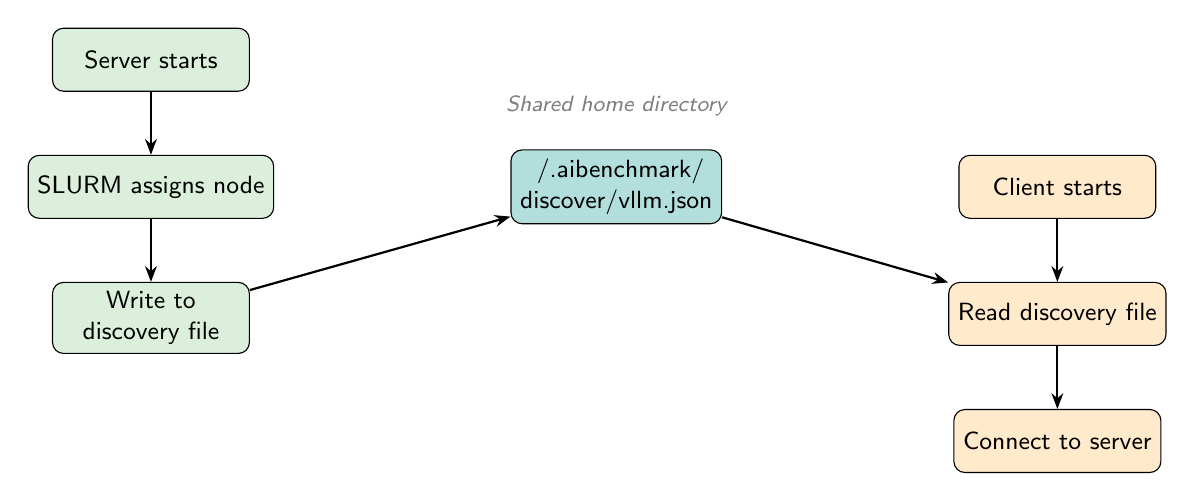
\begin{tikzpicture}[
    node distance=0.8cm,
    block/.style={rectangle, draw, rounded corners, minimum width=2.5cm, minimum height=0.8cm, font=\sffamily\small, align=center},
    arrow/.style={-{Stealth[length=2mm]}, thick},
    note/.style={font=\sffamily\footnotesize\itshape, text=gray}
]

% Server side
\node[block, fill=serverGreen!20] (s1) {Server starts};
\node[block, fill=serverGreen!20, below=of s1] (s2) {SLURM assigns node};
\node[block, fill=serverGreen!20, below=of s2] (s3) {Write to\\discovery file};

% Discovery file
\node[block, fill=discoveryTeal!30, right=3cm of s2] (disc) {~/.aibenchmark/\\discover/vllm.json};

% Client side
\node[block, fill=clientOrange!20, right=3cm of disc] (c1) {Client starts};
\node[block, fill=clientOrange!20, below=of c1] (c2) {Read discovery file};
\node[block, fill=clientOrange!20, below=of c2] (c3) {Connect to server};

% Arrows
\draw[arrow] (s1) -- (s2);
\draw[arrow] (s2) -- (s3);
\draw[arrow] (s3) -- (disc);
\draw[arrow] (c1) -- (c2);
\draw[arrow] (disc) -- (c2);
\draw[arrow] (c2) -- (c3);

% Notes
\node[note, above=0.3cm of disc] {Shared home directory};

\end{tikzpicture}
\caption{Service Discovery Workflow}
\label{fig:discovery}
\end{figure}

\subsection{Service Name Linking}

All recipes for the same service share a common \texttt{service\_name} field:

\begin{lstlisting}[language=yaml, caption={Service Name Consistency Across Recipes}]
# recipes/servers/vllm-server.yaml
name: vllm-server
service_name: vllm  # Discovery key

# recipes/monitors/vllm-monitor.yml
name: vllm-monitor
service_name: vllm  # Same key

# recipes/clients/vllm-simple-test.yaml
name: vllm-simple-test
service_name: vllm  # Same key
\end{lstlisting}

This design allows the client and monitor to automatically find the server without any manual endpoint configuration.


%==============================================================================
\section{Getting Started}
%==============================================================================

This section provides step-by-step instructions for deploying our application on MeluXina.

\subsection{Initial Setup}

\begin{lstlisting}[language=bash, caption={MeluXina Setup Commands}]
# 1. Connect to MeluXina
ssh <username>@meluxina.lxp.lu

# 2. Request an interactive session
salloc -A p200981 -t 02:00:00 -q dev

# 3. Navigate to the repository
cd /path/to/repo

# 4. Run the setup script
./setup.sh

# 5. Configure your SLURM account
export SLURM_ACCOUNT=p200981
\end{lstlisting}

\subsection{Basic Workflow}

\begin{lstlisting}[language=bash, caption={Complete Deployment Workflow}]
# Deploy a vLLM server (auto-registers endpoint)
python -m src.server run --recipe vllm-server
# Output: vllm-server:a1b2c3d4 -> JobID 3757043

# Verify service discovery
python -m src.list_services
# Output: vllm: node=mel2013, ports=[8000]

# Start Prometheus monitoring (auto-discovers server)
python -m src.monitor start --recipe vllm-monitor
# Output: Monitor ID: xyz789, Prometheus: http://mel2014:9090

# Run benchmark (auto-discovers server)
python -m src.client run --recipe vllm-simple-test
# Output: Results saved to ./results/

# Cleanup
python -m src.monitor stop-all
python -m src.server stop-all
python -m src.clear_services
\end{lstlisting}

\subsection{Accessing Prometheus UI}

To access the Prometheus web interface from your local machine:

\begin{lstlisting}[language=bash, caption={SSH Tunnel for Prometheus}]
# From your local machine (new terminal)
ssh -L 9090:mel2014:9090 <username>@meluxina.lxp.lu

# Open in browser
# http://localhost:9090
\end{lstlisting}

%==============================================================================
\section{Benchmarking Results}
%==============================================================================

This section presents the results of comprehensive benchmarking experiments conducted on the MeluXina supercomputer using the project. Four distinct test scenarios were designed to evaluate vLLM inference performance under various workload conditions.



\subsection{Test Scenarios}

Four benchmark recipes were designed to evaluate different aspects of inference performance of vllm. The \textbf{simple test} provided a baseline measurement with 3 concurrent users, 50-token prompts, 20-token generation limits, and 500 milliseconds think time over a 2-minute duration. This test validated basic functionality and established performance baselines. The \textbf{stress test} increased load substantially with 20 concurrent users, 256-token prompts, 128-token generation, and 100 milliseconds think time over 10 minutes. This configuration represented realistic production workloads for conversational AI applications.

The \textbf{high-throughput test} focused on maximum request-per-second capacity by using 50 concurrent users with very short prompts (20 tokens) and minimal generation (10 tokens) with only 50 milliseconds think time. This test evaluated scheduler efficiency and batching capabilities under high request rates. The \textbf{long-context test} evaluated memory scaling and attention mechanism performance with large inputs, using 5 concurrent users with 2048-token prompts and 512-token generation over 10 minutes. Lower concurrency was necessary due to the memory-intensive nature of processing large contexts.

\subsection{Performance Results}

Benchmark results revealed distinct performance characteristics across the four test scenarios. Table~\ref{tab:benchmark-results} summarizes key metrics for each test configuration.

\begin{table}[H]
\centering
\caption{Benchmark Results Summary}
\label{tab:benchmark-results}
\small
\begin{tabular}{lrrrr}
\toprule
\textbf{Test} & \textbf{Throughput} & \textbf{Avg Latency} & \textbf{Max Latency} & \textbf{Requests} \\
& \textbf{(req/s)} & \textbf{(ms)} & \textbf{(ms)} & \\
\midrule
Simple Test & 1.81 & 52.30 & 100.97 & 218 \\
Stress Test & 2.65 & 276.59 & 507.29 & 1593 \\
High-Throughput & 12.02 & 33.10 & 5037.83 & 5000 \\
Long-Context & 0.69 & 945.93 & 1422.34 & 416 \\
\bottomrule
\end{tabular}
\end{table}

The \textbf{simple test baseline} achieved 1.81 requests per second with average latency of 52.30 milliseconds and maximum latency under 101 milliseconds, demonstrating excellent consistency. All 218 requests completed successfully with zero errors. The low latency reflects the minimal computational requirements of the small prompt and generation lengths combined with light concurrent load.

The \textbf{stress test} processed 1593 requests over 10 minutes at 2.65 requests per second with average latency of 276.59 milliseconds. The increased latency compared to the simple test reflects the substantially larger prompt sizes (256 tokens versus 50 tokens) and longer generation lengths (128 tokens versus 20 tokens). Maximum latency remained reasonable at 507.29 milliseconds, indicating good queue management even under sustained concurrent load of 20 users.

The \textbf{high-throughput test} achieved the highest request rate at 12.02 requests per second, processing 5000 total requests with remarkably low average latency of 33.10 milliseconds. This result demonstrates vLLM's efficient batching capabilities when handling many short requests. However, the maximum latency spiked to 5037.83 milliseconds, revealing occasional queueing delays when the system became saturated. This behavior is expected under extreme load and validates the importance of monitoring tail latency in production deployments.

The \textbf{long-context test} exhibited the lowest throughput at 0.69 requests per second and highest average latency at 945.93 milliseconds, which directly reflects the computational cost of processing 2048-token prompts and generating 512-token outputs. Despite the heavy workload, maximum latency remained under 1.5 seconds and all 416 requests completed successfully, demonstrating that the framework can reliably handle memory-intensive inference tasks.

\subsection{Comparative Analysis}

Analyzing performance across test scenarios reveals how workload characteristics affect inference efficiency. \textbf{Throughput scaling} showed clear correlation with request size, where the high-throughput test (short requests) achieved 17.4 times higher throughput than the long-context test (large requests) despite having 10 times more concurrent users. This demonstrates that request size, not just concurrency, determines system capacity. \textbf{Latency scaling} followed expected patterns, with average latency increasing proportionally to prompt length plus generation length. The stress test with medium-sized requests showed 5.3 times higher latency than the simple test, while the long-context test showed 18 times higher latency.

\textbf{Queue management} effectiveness varied by scenario. The simple and stress tests maintained consistent latencies with maximum latencies only 1.9 to 2.0 times higher than average latencies. However, the high-throughput test showed maximum latency 152 times higher than average, indicating that under saturation conditions, some requests experience significant queueing delays while most requests are processed quickly. This bimodal distribution is characteristic of systems operating at capacity limits. \textbf{Reliability} remained excellent across all scenarios, with 100\% success rates and zero errors even under extreme load conditions totaling 7,227 completed requests.

\subsection{Time-Series Analysis}



Prometheus monitoring data collected during the stress test provides insight into system behavior over time. Data shows average generation throughput measured in tokens per second. After an initial ramp-up period, throughput stabilized around 300 tokens per second, demonstrating consistent performance throughout the 10-minute test duration. The relatively flat profile indicates efficient resource utilization without degradation over time.

GPU cache usage percentage exhibited periodic fluctuations between near-zero and 0.014\% as shown in monitoring data, which reflects vLLM's dynamic cache management. These values confirm that the opt-125m model with specified context lengths did not stress memory capacity.

Request queue depths remained low throughout testing, with running requests typically between 1 and 3 concurrent operations and waiting requests occasionally spiking to 5 during burst periods. These patterns confirm that the CPU allocation provided sufficient compute capacity to process incoming requests without building large backlogs. 



%==============================================================================
\section{Conclusion}
%==============================================================================

Our application provides a comprehensive solution for deploying, monitoring, and benchmarking AI inference services on HPC clusters. The framework addresses key challenges in managing containerized AI workloads in SLURM environments through a modular architecture with clear separation of concerns, automatic service discovery that eliminates manual endpoint management, recipe-based configuration for reproducible deployments, integrated Prometheus monitoring with automatic target resolution, and flexible benchmarking capabilities with configurable workload patterns.

The framework has been successfully deployed and tested on the MeluXina supercomputer, demonstrating its effectiveness for managing AI inference workloads in production HPC environments. Comprehensive benchmarking experiments validated the framework's capabilities across diverse workload scenarios, processing over 7,200 inference requests with 100\% success rates. Performance results showed that the framework efficiently handles workloads ranging from simple validation tests to high-throughput scenarios processing 12 requests per second, as well as memory-intensive long-context inference with multi-kilobyte prompts.

Time-series monitoring data confirmed consistent throughput and resource utilization throughout extended test runs, demonstrating the framework's reliability for sustained production workloads. The declarative recipe system proved effective for defining reproducible benchmarks with varying concurrency levels, request sizes, and workload patterns.



\end{document}